%!TEX root = main.tex
\chapter{Resultados y conclusiones}
En este capítulo se presentan los resultados obtenidos en el desarrollo de esta
memoria.
En la sección~\ref{sec:datos} se muestra información y estadísticas de los datos
analizados como son las fechas, los tipos de consultas, los \emph{endpoint} más
utilizados y otra información relevante del proyecto Bio2RDF.

La sección~\ref{sec:res} presenta los resultados obtenidos tanto de la
extracción y creación del grafo RDF como del cálculo de su centralidad. Con
estos datos se hacen los análisis y las comparaciones pertinentes.

Por último, en la sección~\ref{sec:con}, se enuncian las conclusiones generales
obtenidas junto a una comparación de ellas con lo que se espera del proyecto
Bio2RDF. Además se evidencian los problemas detectados y se genera una lista de
posibles mejoras y trabajo futuro con respecto a este tema.


\section{Datos analizados}\label{sec:datos}
Para el análisis llevado a cabo en este trabajo se dispuso de 12Gb de consultas
almacenadas en 57.016 archivos de registros obtenidos del proyecto Bio2RDF.
Cada linea de un archivo de registro almacena una consulta y metadatos 
relacionados a ella en forma de diccionario \tt{json}. En esta sección se
analizarán estos datos.

Con respecto a la fecha, las consultas fueron efectuadas desde el 05 de mayo del
2013 hasta el 18 de septiembre del 2015.
La figura~\ref{fig:dates} muestra una gráfica de la distribución de consultas
realizadas al proyecto en este periodo.
Para el análisis debemos tener en cuenta que los datos del mes inicial y final
no se registraron completamente.

\begin{figure}[ht]
  \begin{tikzpicture}
    \begin{axis}[
        xlabel=Fecha (año-mes), ylabel=Número de consultas,
        xticklabel style={rotate=90,anchor=near xticklabel},
        width=\textwidth,height=6cm,compat=1.9,
        date coordinates in=x,date ZERO=2013-05-01,
        ymin=0,ymax=1500000, xticklabel=\year-\month,
        xmin=2013-04-01,xmax=2015-10-01]
      \addplot table [x=date,y=value,col sep=comma]{data/mdates.csv};
    \end{axis}
  \end{tikzpicture}
  \caption{Fechas de las consultas.}\label{fig:dates}
\end{figure}

Los registros disponen de una total de 12.881.518 consultas hechas por 9.818 IPs
diferentes, las cuales realizaron entre 1 y 2.831.912 peticiones cada una.

En la figura~\ref{fig:ips} se muestra la cantidad de IPs que realizan hasta
cierto número de consultas.
Como podemos ver en ella, la mayoría de las IPs efectuó entre 1 y 100 consultas,
pero su aporte al total es bajo (menos de 1\%), de hecho, las 23 IPs con mayor
cantidad de consultas (más de $10^5$) aportan cerca del 80\% del total, el
detalle de estas IPs puede ser visto en la tabla~\ref{tab:ips}.

\begin{figure}[ht]
  \begin{tikzpicture}
    \begin{axis}[ybar, ymin=0, ymax=4500,
        xlabel=Número de consultas, ylabel=Número de IPs,compat=1.9,
        width=\textwidth,height=6cm,
        xtick=data,
        xticklabels={{$1$},{$10$},{$10^2$},{$10^3$},{$10^4$},{$10^5$},{$10^6$},{$10^7$}},
        nodes near coords,
        nodes near coords align={vertical}]
    \addplot table [x expr=\coordindex,y=value,col sep=comma]{data/ip.csv};
    \end{axis}
  \end{tikzpicture}
  \caption{Cantidad de consultas por IP.}\label{fig:ips}
\end{figure}

\begin{table}[ht]
  \centering
  \begin{tabular}{|r|l|l|l|} \hline
    \bf{Consultas} & \bf{IP} & \bf{Pais} & \bf{Instituación} \\\hline
    121646  & 150.214.40.112  & España         
                   & Centro Informatico Cientifico de Andalucia\\\hline
    129006  & 37.6.165.5      & Grecia         
                   & Desconocido\\\hline
    134178  & 79.107.219.216  & Grecia         
                   & Desconocido\\\hline
    141036  & 134.160.214.42  & Japón          
                   & RIKEN\\\hline
    143496  & 134.117.221.16  & Canadá         
                   & Carleton University\\\hline
    150236  & 155.185.49.66   & Italia         
                   %& Universita Degli Studi Di Modena E Reggio Emilia\\\hline
                   & Degli Studi Di Modena E Reggio Emilia\\\hline
    153794  & 134.117.108.151 & Canadá         
                   & Carleton University\\\hline
    166286  & 24.130.52.25    & EEUU 
                   & Desconocido\\\hline
    167895  & 134.117.108.111 & Canadá         
                   & Carleton University\\\hline
    217148  & 134.117.108.158 & Canadá         
                   & Carleton University\\\hline
    229289  & 173.178.48.100  & Canadá         
                   & Desconocido\\\hline
    232020  & 140.203.154.5   & Irlanda        
                   & National University of Ireland Galway\\\hline
    233677  & 159.90.11.58    & Venezuela      
                   & Universidad Simón Bolívar\\\hline
    238541  & 134.117.108.159 & Canadá         
                   & Carleton University\\\hline
    251789  & 146.155.115.75  & Chile          
                   & Pontificia Universidad Católica de Chile\\\hline
    259143  & 140.203.154.6   & Irlanda        
                   & National University of Ireland Galway\\\hline
    304598  & 133.11.132.151  & Japón          
                   & University of Tokyo\\\hline
    342553  & 140.203.154.11  & Irlanda        
                   & National University of Ireland Galway\\\hline
    478989  & 129.26.128.185  & Alemania       
                   & Fraunhofer-Gesellschaft\\\hline
    801417  & 129.26.131.1    & Alemania       
                   & Fraunhofer-Gesellschaft\\\hline
    1130035 & 134.117.221.14  & Canadá         
                   & Carleton University\\\hline
    1391974 & 171.65.32.83    & EEUU 
                   & Stanford University\\\hline
    2831912 & 132.203.117.5   & Canadá         
                   & Universite Laval\\\hline
  \end{tabular}
  \caption{IPs con más consultas.}\label{tab:ips}
\end{table}

En la tabla~\ref{tab:ips} además podemos notar como la mayoría de las
instituciones a las cuales pertenecen las IPs son universidades o centros de
investigación.

Este fenómeno era de esperar ya que, aunque estamos hablando de datos abiertos,
la naturaleza de ellos los hace útiles sólo para el publico especializado, ya
sea para la investigación biológica o en la relacionada a la informática.

En la figura~\ref{fig:size} se presenta una gráfica de la cantidad de consultas
registradas y el peso de la respuesta correspondiente. Estas respuestas van
desde el rango de los kilobytes (entre $2^{10}$ y $2^{19}$), pasando por los
megabutes (entre $2^{20}$ y $2^{29}$) y llegando incluso a los gigabytes (entre
$2^{30}$ y  $2^{39}$).
Como podemos ver en ella, la mayor cantidad de consultas tiene retornos de unos
pocos kilobytes o menos.
Generalmente esto corresponde a tablas con pocas filas (o ninguna),
identificadores de retorno vacío (\tt{\# Empty NT}) o resultados de operaciones
más complejas (como calcular promedios, contar recursos según ciertos filtros,
etc).

La mayor concentración se encuentra en el rango de los kilobytes y al principio
de los megabytes.
Pocas consultas retornan más de un gigabyte de datos y posiblemente
corresponden a consultas como la de la figura~\ref{fig:exbigq} y similares que
retornan toda la base de datos.

\begin{figure}[ht]
  \begin{tikzpicture}
    \begin{axis}[
        xlabel=Tamaño de la respuesta (en bytes), ylabel=Número de consultas,
        width=\textwidth,height=6cm,compat=1.9,
        xticklabel={2\textsuperscript{\pgfmathprintnumber{\tick}}},
        ymode=log,
        xmin=8,xmax=32]
      \addplot table [x=exp,y=n,col sep=comma]{data/size.csv};
    \end{axis}
  \end{tikzpicture}
  \caption{Tamaño de las respuestas registradas.}\label{fig:size}
\end{figure}

Como se explica en la sección~\ref{d:emc} los registros almacenan el tipo de
consulta hecha al servidor en los atributos \tt{DESCRIBE}, \tt{ASK},
\tt{CONSTRUCT} y \tt{SELECT}. Generalmente se marca con un $1$ cuando la
consulta es de ese tipo y con un $0$ en caso contrario pero existen dos casos
particulares.
Si la consulta presenta un error todos los atributos se marcarán como una cadena
de caracteres vacía, y si no se puede determinar el tipo, todos los atributos
serán 0. Si sucede lo último diremos que la consulta es de tipo ``desconocido''.

\begin{figure}[ht]
  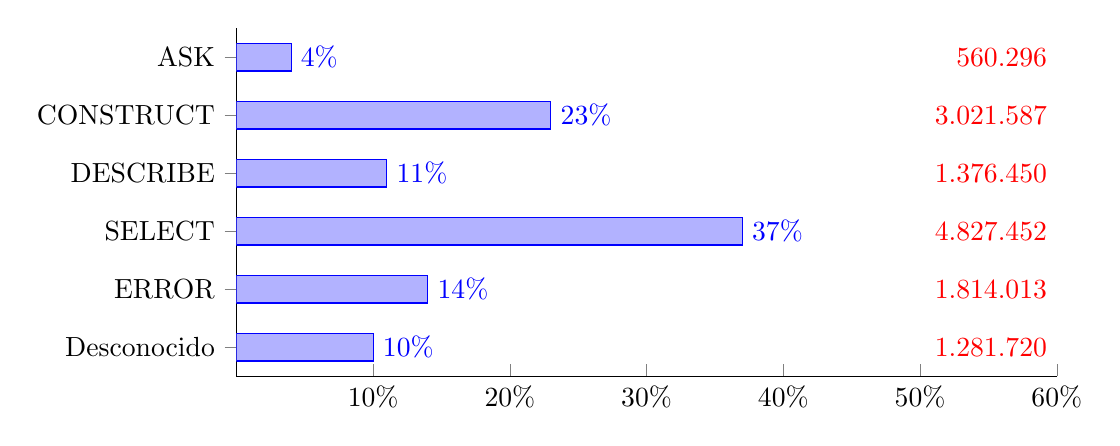
\begin{tikzpicture}
    \begin{axis}[axis lines*=left, xbar, width=12cm, height=6cm, xlabel={},
      symbolic y coords={Desconocido, ERROR, SELECT, DESCRIBE, CONSTRUCT, ASK },
      ytick=data, xmin=0, xmax=0.6, nodes near coords,
      nodes near coords align={horizontal},xtick={0.1, 0.2, 0.3, 0.4, 0.5, 0.6},
      xticklabel={\pgfmathparse{\tick*100}\pgfmathprintnumber{\pgfmathresult}\%},
      point meta={x*100},
      nodes near coords={\pgfmathprintnumber\pgfplotspointmeta\%},
      nodes near coords align={horizontal}]
      \addplot coordinates
      {(0.37,SELECT) (0.23,CONSTRUCT) (0.11,DESCRIBE)
       (0.04,ASK) (0.10,Desconocido) (0.14,ERROR)};

      \node[red,left] at (axis cs:0.6,SELECT)      {4.827.452};
      \node[red,left] at (axis cs:0.6,CONSTRUCT)   {3.021.587};
      \node[red,left] at (axis cs:0.6,ASK)         {560.296};
      \node[red,left] at (axis cs:0.6,ERROR)       {1.814.013};
      \node[red,left] at (axis cs:0.6,DESCRIBE)    {1.376.450};
      \node[red,left] at (axis cs:0.6,Desconocido) {1.281.720};
    \end{axis}
  \end{tikzpicture}
  \caption{Tipo de consultas realizadas.}\label{fig:qtype}
  \vspace{-.2cm}
  \caption*{En rojo el total de consultas por tipo.}
\end{figure}

La figura~\ref{fig:qtype} presenta los tipos de consultas almacenadas en los
registros. Como podemos notar el tipo predominante es \tt{SELECT} seguido de
\tt{CONSTRUCT}. Este es un resultado esperado debido a que la forma más natural
de consultar información a una base de datos es mediante \tt{SELECT} ya que este
retorna la información en una tabla, formato fácil de leer por los humanos.

La aparición de \tt{CONSTRUCT} en segundo lugar denota que gran parte de los
usuarios del proyecto Bio2RDF utilizan los datos directamente como  triples RDF,
posiblemente ya que esto facilita el manejo de los datos por parte de las
computadoras.

Las consultas tipo \tt{ASK} son las menos populares, lo que muestra que
generalmente un usuario prefiere utilizar \tt{SELECT} o \tt{CONSTRUCT} y manejar
un posible retorno vacío, que preguntar si existen los datos primero (aunque
\tt{ASK} sea más rápido, si se requiere obtener los datos después de una
respuesta afirmativa se necesitará una consulta adicional).

\begin{figure}[ht]
  \begin{tikzpicture}
    \begin{axis}[ybar, ymin=0, ymax=38, xtick=data,
        ylabel=Porcentaje del total de consultas,
        flexible xticklabels from table={data/t10endp.csv}{label}{col sep=comma},
        width=\textwidth,height=6cm,compat=1.9,
        xticklabel style={rotate=90,anchor=near xticklabel},
        yticklabel={\pgfmathprintnumber{\tick}\%},
        nodes near coords={\small\pgfmathprintnumber\pgfplotspointmeta\%},
        nodes near coords align={vertical}]
      \addplot table[x expr=\coordindex,y=p]{\tableendp};
    \end{axis}
  \end{tikzpicture}
  \caption{Diez \emph{endpoint} más consultados.}\label{fig:t10endp}
\end{figure}

Por último, la figura~\ref{fig:t10endp} presenta los diez \emph{endpoint} más
consultados en el proyecto Bio2RDF. La barra ``Otros'' agrupa las consultas de
los 35 \emph{endpoint} con menos de $3,5\%$ de consultas cada uno. Cabe destacar
que si bien la consulta se dirige a cierto \emph{endpoint}, los resultados de la
misma pueden ir más allá de este dominio pues una de las características del
proyecto Bio2RDF es la existencia de enlaces entre las diferentes bases de datos
que componen el proyecto.

\section{Resultados obtenidos}\label{sec:res}
En esta sección se presentan los resultados obtenidos de la ejecución de los
programas descritos en el capítulo~\ref{c:desarrollo} junto a pasos 
adicionales y consideraciones para optimizar el proceso.

En la sección~\ref{sec:res:extr} se muestran estadísticas del proceso de
extracción y modificación de consultas, mientras que en la
sección~\ref{sec:res:obt} se hace lo mismo con el proceso de obtención de
triples.
Por último, en la sección~\ref{sec:res:cent} se presentan los resultados del
calculo de centralidad y datos relacionados a ellos.

\subsection{Extracción y modificación de consultas}\label{sec:res:extr}
Para recrear la porción de la base de datos consultada por los usuarios se
ejecutó el programa descrito en el algoritmo~\ref{alg:extract} sobre todos los
archivos, generando las consultas \tt{CONSTRUCT} correspondientes.

En este proceso 3.750.759 consultas fueron omitidas. Estas corresponden a la
suma de las consultas tipo \tt{ASK}, \tt{DESCRIBE} y \tt{ERROR} de la
figura~\ref{fig:qtype}.

Las 9.130.759 consultas restantes pasaron por el proceso de modificación en el
cual se crearon 9.212.229 consultas y 838 tuvieron errores de procesamiento
(el $0.004\%$).
Como podemos notar se obtuvieron 82.308 consultas más que las procesadas
correctamente, esto es debido a la separación de las clausulas \tt{OPTIONAL} en
consultas diferentes, como es descrito en la sección~\ref{d:emc}.

De las consultas creadas 2.908.304 fueron marcadas como consultas con solo
variables, las cuales fueron guardadas en un archivo diferente para pasar por
filtros adicionales. 
Además, del análisis de las consultas marcadas con errores, se descubrió que
831 de ellas presentan problemas con su codificación ya que fueron guardadas en
formato de código porciento. Otras 6 consultas poseen errores de sintaxis
irrecuperables y solo 1 era valida pero no pudo ser procesada.

\subsection{Obtención de los triples}\label{sec:res:obt}
Para obtener los triples RDF consultados por los usuarios debemos ejecutar las
consultas creadas en el \emph{endpoint} a analizar, en este caso la última
versión de DrugBank, como se describe en la sección~\ref{d:cg}.

Para evitar hacer más consultas de las necesarias se omitieron las consultas
repetidas y, de las consultas con solo variables, se ejecutaron solo aquellas
que poseen algún filtro (\tt{FILTER}). De esta manera se redujo el número de
consultas a 7.014.088.

De este proceso se obtuvieron los siguientes resultados:
\begin{itemize}
  \item
    6640609 consultas tuvieron un retorno vacío (\tt{\#Empty NT}), esto
    corresponde al $94.6\%$ de las consultas analizadas.
    Creemos que la razón principal del por qué estas consultas no retornan
    información es debido a que se requieren datos que no están en DrugBank y
    por ello no se pueden crear los triples necesarios.
    %Para distinguir entre las consultas que recaen en el fenómeno anterior y
    %aquellas que realmente no tienen respuesta se podrían consultar con ASK los
    %mismos triples a todos las bases de datos de Bio2RDF y así determinar
    %cuales realmente deberían dar vacío. Este proceso es demasiado costoso y
    %por ello no se realizó.
  \item
    279892 consultas retornaron datos, esto corresponde a un $4\%$ del total de
    consultas ejecutadas. Este resultado es cercano al $6.6\%$ de consultas que
    DrugBank presenta según la figura~\ref{fig:t10endp}, la diferencia puede ser
    atribuida principalmente a dos factores: el tipo de consulta y aquellas
    consultas que piden datos de más de una base de datos.
  \item
    93587 consultas resultaron en error, esto corresponde a un $1,33\%$, de
    ellas:
    \begin{itemize}
      \item
        86402 son \tt{HTTP Error 500: SPARQL Request Failed}, que significa que
        ocurrió un error interno en el servidor \emph{virtuoso}, esto puede ser
        debido a que se sobrepasó el tiempo máximo de procesamiento o que se
        piden más datos de los permitidos.
      \item 
        7029 son \tt{HTTP Error 400: Bad Request}, que evidencia una consulta
        SPARQL mal formulada, este error es puede ser atribuido a posibles
        errores en el proceso de creación y modificación de las consultas.
      \item
        156 son \tt{HTTP Error 404: File not found}, que es causado cuando un
        recurso que se pide no es encontrado.
    \end{itemize}
\end{itemize}

\subsection{Centralidad}\label{sec:res:cent}
En este punto ya tenemos todos los datos necesarios en un archivo N-Triples. Con
el algoritmo~\ref{alg:convert} estos datos se convierten en un grafo, en este
caso el orden del grafo creado es de 6.364.209, del cual se calcula la
centralidad según el algoritmo~\ref{alg:degree} y el~\ref{alg:bet}.

Los distintos tipos de centralidad denotan diferentes significados para un grafo
RDF.
Se podría decir que las centralidades de grado mostrarán los recursos que son
más usados como $sujetos$ u $objetos$ en las consultas realizadas, mientras que
la intermediación le dará importancia a aquellos recursos que participan como
nexo entre los diferentes triples de una consulta.

Supongamos una consulta como:
\begin{center}
  \tt{SELECT * WHERE \{?a ?b ?c . ?c ?d ?e .\} LIMIT 1}
\end{center}
Para la centralidad de grado entrante \tt{?c} y \tt{?e} serán los elementos más
centrales, pues participan como $objeto$ en las consultas, mientras que para el
grado saliente lo serán \tt{?a} y \tt{c} (ya que son los $sujetos$).
Se podría decir que la centralidad de grado saliente nos muestra cuales son los
recursos más estudiados mientras que la entrante valora las cualidades de los
mismos.

Por otro lado, para la intermediación el recurso más central será $?c$, ya que
este participa como nexo entre los dos triples, pero debemos tener en
consideración que la intermediación también le da valor a aquello a lo que se le
está haciendo nexo.
Cuando obtenemos los resultados de muchas consultas, la intermediación será
mayor en aquellos nodos que son nexos vitales para la obtención de la mayoría de
los datos.
Así, un resultado por intermediación no da la información más estudiada en la
base de datos, sino que aquellos vínculos que fueron más necesarios para
obtenerla.

\subsubsection{Centralidad de grado entrante}
\begin{itemize}
  \item 3.819.971 ($60\%$) obtuvieron una centralidad de 0, de los cuales:
    \begin{itemize}
      \item 3.803.439 ($59,76\%$) son recursos anónimos.
      \item 16.532 ($0,25\%$) son URIs.
    \end{itemize}
  \item 2.544.238 ($39,97\%$) tienen centralidad entre 1 y 1.453.738, de los cuales:
    \begin{itemize}
      \item 1.377.801 ($21,64\%$) son recursos de XMLSchema.
      \item 595.782 ($9,35\%$) son son cadenas de caracteres.
      \item 507.516 ($7,97\%$) son URIs.
      \item 63.139 ($0,99\%$) son recursos anónimos.
    \end{itemize}
  \item La centralidad acumulada de todos los nodos es de 9.773.000.
  \item 
    Los recursos parte del vocabulario (\tt{.*\_vocabulary.*}) aportan un 
    $51,51\%$ de la centralidad acumulada total.
  \item
    Recursos no pertenecientes a Bio2RDF aportan un $32,72\%$ incluyendo a OWL 
    ($0,698\%$).
  \item 
    Recursos parte de Bio2RDF que no son parte del vocabulario contribuyen con
    un $16,44\%$ de la centralidad total. La tabla~\ref{tab:idct5} presenta un
    detalle de los más centrales.
\end{itemize}

La distribución de esta centralidad se puede ver en la
tabla~\ref{tab:idcres}\footnote{Se omite el prefijo \tt{http://bio2rdf.org/} de
la columna `Recurso' por conveniencia.}.
La columna `Valor' indica la centralidad entrante relativa a la acumulada del
grafo completo.
Como podemos notar, los recursos más centrales son parte del vocabulario y casi
un $50\%$ de la centralidad total está en los primeros 10 nodos.

\begin{table}[ht]
  \centering
  \begin{tabular}{|r|l|r|}\hline
    \bf{Puesto} & \bf{Recurso} & \bf{Valor} \\\hline
     1 & drugbank\_vocabulary:Drug-Drug-Interaction				 	 & $14.87\%$ \\\hline
     2 & pubmed\_vocabulary:Resource												 & $4.72\%$ \\\hline
     3 & drugbank\_resource:bio2rdf.dataset.drugbank.R4			 & $4.31\%$ \\\hline
     4 & drugbank\_vocabulary:Resource											 & $3.97\%$ \\\hline
     5 & drugbank\_vocabulary:Pharmaceutical								 & $3.80\%$ \\\hline
     6 & drugbank\_vocabulary:Dosage												 & $3.65\%$ \\\hline
     7 & drugbank\_vocabulary:Drug													 & $3.39\%$ \\\hline
     8 & uniprot\_vocabulary:Resource												 & $3.32\%$ \\\hline
     9 & "drugbank\_resource"$\wedge\wedge$XMLSchema\#string & $3.21\%$ \\\hline
    10 & drugbank\_resource:60e815570c1c11cef30f3fff503d6264 & $1.63\%$ \\\hline
    11-100 		& & $14.51\%$ \\\hline
    101-1000  & & $5.99\%$ \\\hline
    1001--    & & $28.52\%$ \\\hline
  \end{tabular}
  \caption{Resultados de la centralidad de grado entrante.}\label{tab:idcres}
\end{table}

La tabla~\ref{tab:idct5} por su parte muestra los cinco recursos más centrales
por grado entrante que no son parte del vocabulario.

\begin{table}[h]
  \centering
  \begin{tabular}{|r|l|r|}\hline
    \bf{Puesto} & \bf{Recurso} & \bf{Valor} \\\hline
    1~~(3) & drugbank\_resource:bio2rdf.dataset.drugbank.R4			 & $4.31\%$ \\\hline
    2 (10) & drugbank\_resource:60e815570c1c11cef30f3fff503d6264 & $1.63\%$ \\\hline
    3 (16) & uniprot:O95477                                      & $0.51\%$ \\\hline
    4 (24) & drugbank\_resource:c78f5087e52c969400b9d748ae4a9485 & $0.21\%$ \\\hline
    5 (82) & drugbank\_resource:e0783716ac65b1e931488d76b4d988fd & $0.07\%$ \\\hline
  \end{tabular}
  \caption{Recursos no parte del vocabulario por grado entrante.}
  \label{tab:idct5}
\end{table}

El recurso \tt{bio2rdf.dataset.drugbank.R4} es una etiqueta de la fuente de los
datos, referente a que los datos provienen de la \emph{release} 4 de Bio2RDF.
El recurso \tt{60e815570c1c11cef30f3fff503d6264} hace referencia a 
ChemAxon\footnote{\url{https://www.chemaxon.com/}},
mientras que el \tt{c78f5087e52c969400b9d748ae4a9485} es 
ALOGPS\footnote{\url{http://www.vcclab.org/lab/alogps/}}, ambas aplicaciones
informáticas que figuran como fuente de algunos datos de DrugBank.
El recurso \tt{uniprot:O95477} tiene como título \emph{ATP-binding cassette
sub-family A member 1}, también conocido como el gen ABCA1, ésta implicado en
la homeostasis del colesterol. Por último el recurso 
\tt{e0783716ac65b1e931488d76b4d988fd} es la clasificación de una droga como
componente orgánico.

Como podemos notar, los recursos más centrales son aquellos parte del
vocabulario y la fuente de los datos.
Solo un gen logra entrar a la lista de los mejores según esta medida.

\subsubsection{Centralidad de grado saliente}
\begin{itemize}
  \item 2.089.942 ($32,83\%$) obtuvieron una centralidad de 0, de los cuales:
    \begin{itemize}
      \item 1.377.801 ($21,64\%$) son recursos de XMLSchema.
      \item 595.782 ($9,36\%$) son son cadenas de caracteres.
      \item 101.570 ($1,59\%$) son URIs.
      \item 14.789 ($0,23\%$) son recursos anónimos.
    \end{itemize}
  \item
    4.274.267 ($67,16\%$) tienen centralidad entre 1 y 100.001, de los cuales:
    \begin{itemize}
      \item 3.851.789 ($60,52\%$) son recursos anónimos.
      \item 422.478 ($6,63\%$) son URIs.
    \end{itemize}
  \item La centralidad acumulada de todos los nodos es de 9.773.000.
  \item 
    Los recursos parte del vocabulario (\tt{.*\_vocabulary.*}) aportan un 
    $1,83\%$ de la centralidad acumulada total.
  \item
    Recursos no pertenecientes a Bio2RDF aportan un $39,62\%$ incluyendo OWL 
    ($0,008\%$) y recursos anónimos ($39,41\%$).
  \item 
    Recursos parte de Bio2RDF que no son parte del vocabulario contribuyen con
    un $58,54\%$ de la centralidad total.
\end{itemize}

La tabla~\ref{tab:odcres} presenta los nodos con mayor centralidad de grado
saliente.
Como podemos notar, el recurso más central es ordenes de magnitud más grande
que los recursos que lo siguen, pero aún así no acumula gran porcentaje de la
centralidad total.
Se ve una distribución bastante homogénea pues el $99.98\%$ de los nodos (1001-)
acumulan el $95.52\%$ de la centralidad total.

\begin{table}[ht]
  \centering
  \begin{tabular}{|r|l|r|}\hline
    \bf{Puesto} & \bf{Recurso} & \bf{Valor} \\\hline
     1 & \tt{http://bio2rdf.org/drugbank\_target:4512} & $1.023\%$ \\\hline
     2 & \tt{http://bio2rdf.org/drugbank:DB01050}      & $0.062\%$ \\\hline
     3 & \tt{http://bio2rdf.org/drugbank:DB00316}      & $0.034\%$ \\\hline
     4 & \tt{http://bio2rdf.org/drugbank:DB00281}      & $0.029\%$ \\\hline
     5 & \tt{http://bio2rdf.org/drugbank:DB00388}      & $0.024\%$ \\\hline
     6 & \tt{http://bio2rdf.org/drugbank:DB00514}      & $0.023\%$ \\\hline
     7 & \tt{http://bio2rdf.org/drugbank:DB00563}      & $0.021\%$ \\\hline
     8 & \tt{http://bio2rdf.org/drugbank:DB00898}      & $0.019\%$ \\\hline
     9 & \tt{http://bio2rdf.org/drugbank:DB00874}      & $0.018\%$ \\\hline
    10 & \tt{http://bio2rdf.org/drugbank:DB00152}      & $0.017\%$ \\\hline
    11-100 		& & $0.759\%$ \\\hline
    101-1000  & & $2.419\%$ \\\hline
    1001--    & & $95.52\%$ \\\hline
  \end{tabular}
  \caption{Resultados de la centralidad de grado saliente.}\label{tab:odcres}
\end{table}

Otro factor a considerar es que entre los recursos más centrales por grado
saliente no se encuentran aquellos que forman parte del vocabulario, en vez de
ello encontramos drogas como el ibuprofeno (\tt{DB01050}), el paracetamol
(\tt{DB00316}), la lidocaína (\tt{DB00281}), la fenilefrina (\tt{DB00388}),
el dextrometorfano (\tt{DB00514}), el metotrexato (\tt{DB00563}), el etanol
(\tt{DB00898}), la guaifenesina (\tt{DB00874}) y la tiamina (\tt{DB00152}).
Lamentablemente para \tt{drugbank\_target:4512} no hay información disponible.

Los resultados evidencian la popularidad de ciertas drogas como solución a las
consultas hechas por los usuarios. 

\subsubsection{Intermediación}
\begin{itemize}
  \item 5.909.923 ($92.86\%$) obtuvieron una centralidad de 0, de los cuales:
    \begin{itemize}
      \item 3.818.228 ($60\%$) son recursos anónimos.
      \item 1.377.802 ($21.64\%$) son recursos de XMLSchema.
      \item 595.782 ($9.36\%$) son son cadenas de caracteres.
      \item 118111 ($1.85\%$) son URIs.
    \end{itemize}
  \item
    454.286 ($7.14\%$) tienen centralidad entre $0.00361$ y 1.378.576.128, de
    los cuales:
    \begin{itemize}
      \item 405.936 ($6.37\%$) son URIs.
      \item 48.350 ($0.76\%$) son recursos anónimos.
    \end{itemize}
  \item La centralidad acumulada de todos los nodos es de 2.401.290.198,71.
  \item
    La centralidad media es de $377.31$, 23665 ($0.37\%$) nodos sobrepasan
    la media.
  \item 
    Los recursos parte del vocabulario (\tt{.*\_vocabulary.*}) aportan un 
    $85,23\%$ de la centralidad acumulada total.
  \item
    Recursos no pertenecientes a Bio2RDF aportan un $3.84\%$ incluyendo OWL 
    ($3.48\%$).
  \item 
    Recursos parte de Bio2RDF que no son parte del vocabulario contribuyen con
    un $10.92\%$ de la centralidad total. La tabla~\ref{tab:bet5} presenta los
    cinco más centrales.
\end{itemize}

La tabla~\ref{tab:betres} presenta los diez nodos más centrales según su valor
de intermediación y una comparación con el valor del resto del grafo.
Como podemos notar, los nodos más centrales nuevamente suelen ser aquellos parte
del vocabulario, además, casi toda la centralidad está acumulada en los primeros
nodos.

\begin{table}[ht]
  \centering
  \begin{tabular}{|r|l|r|}\hline
    \bf{Puesto} & \bf{Recurso} & \bf{Valor} \\\hline
     1 & drugbank\_vocabulary:Drug-Drug-Interaction          & $57.4\%$ \\\hline
     2 & drugbank\_vocabulary:Drug                           & $12.6\%$ \\\hline
     3 & uniprot:O95477                                      & $4.73\%$ \\\hline
     4 & drugbank\_vocabulary:Resource                       & $3.21\%$ \\\hline
     5 & drugbank\_vocabulary:Target                         & $2.17\%$ \\\hline
     6 & \tt{http://www.w3.org/2002/07/owl\#Class}           & $2.08\%$ \\\hline
     7 & drugbank\_vocabulary:Pharmaceutical                 & $2.04\%$ \\\hline
     8 & drugbank\_vocabulary:Dosage                         & $2.00\%$ \\\hline
     9 & \tt{http://www.w3.org/2002/07/owl\#ObjectProperty}  & $1.07\%$ \\\hline
    10 & drugbank\_resource:60e815570c1c11cef30f3fff503d6264 & $0.92\%$ \\\hline
    11-100 		& & $6.04\%$ \\\hline
    101-1000  & & $1.96\%$ \\\hline
    1001--    & & $3.02\%$ \\\hline
  \end{tabular}
  \caption{Resultados de la intermediación.}\label{tab:betres}
\end{table}

La tabla~\ref{tab:bet5} muestra los cinco recursos más centrales por
intermediación que no son parte del vocabulario.

\begin{table}[h]
  \centering
  \begin{tabular}{|r|l|r|}\hline
    \bf{Puesto} & \bf{Recurso} & \bf{Valor} \\\hline
    1~~(3) & uniprot:O95477                                      & $4.733\%$ \\\hline
    2 (10) & drugbank\_resource:60e815570c1c11cef30f3fff503d6264 & $0.928\%$ \\\hline
    3 (24) & drugbank\_resource:c78f5087e52c969400b9d748ae4a9485 & $0.125\%$ \\\hline
    4 (27) & drugbank:DB00157                                    & $0.066\%$ \\\hline
    5 (32) & drugbank:DB00898                                    & $0.044\%$ \\\hline
  \end{tabular}
  \caption{Recursos no parte del vocabulario por intermediación.}
  \label{tab:bet5}
\end{table}

Entre estos recursos nuevamente encontramos el gen ABCA1 (\tt{uniprot:O95477}),
la fuente de datos ChemAxon (\tt{60e815570c1c11cef30f3fff503d6264}) y ALOGPS
(\tt{c78f5087e52c969400b9d748ae4a9485}) y por último la droga
NADH (\tt{DB00157}) y el etanol (\tt{DB00898}).

\subsubsection{Comparación}
La figura~\ref{fig:compcent} presenta una comparación en la centralidad relativa
de los diez nodos más centrales según la centralidad de grado entrante (IDC), la
saliente (ODC) y la intermediación (BC).
\begin{figure}[h]
  \begin{tikzpicture}
    \begin{axis}[
        xlabel=Nodos más centrales, ylabel=\% de la centralidad total,
        ymode=log,
        log ticks with fixed point,
        width=\textwidth,height=6cm,compat=1.9]
      \addplot table [x=n, y=idc,col sep=comma]{data/best10.csv};
      \addlegendentry{IDC}
      \addplot table [x=n, y=odc,col sep=comma]{data/best10.csv};
      \addlegendentry{ODC}
      \addplot table [x=n, y=bet,col sep=comma]{data/best10.csv};
      \addlegendentry{BC}
    \end{axis}
  \end{tikzpicture}
  \caption{Comparación de centralidad para los primeros 10 nodos.}
  \vspace{-.2cm}
  \caption*{
    Para BC el nodo más central es un orden de magnitud más grande que aquellos
    que lo siguen, muy pocos nodos logran centralidades altas.
    Para ODC el nodo más central es bastante más central que aquellos que lo
    siguen, pero en general la centralidad se acumula en los primeros diez
    nodos.
    Por último, para IDC el nodo más central acumula cerca del $1\%$ del total,
    pero el resto está disperso en todo el grafo.
  }
  \label{fig:compcent}
\end{figure}

La intermediación presenta la distribución de centralidad más desigual, el
primer nodo acumula más del $50\%$ del total, mientras que los siguientes decaen
rápidamente, esto demuestra que existen puntos críticos en la búsqueda de datos.
Por su parte la centralidad de grado entrante presenta varios nodos con
centralidades relativamente altas, lo que evidencia la existencia de una serie
de propiedades que son generalmente buscadas por sobre las demás.
Finalmente, la centralidad de grado saliente posee la distribución más
homogénea, lo que es evidencia de que la mayoría de las drogas (en especial la
más central) suelen estar presentes en las respuestas obtenidas.

Por su parte, la figura~\ref{fig:comptype} grafica la centralidad relativa de
los nodos que pertenecen al vocabulario, los recursos de Bio2RDF (drogas, genes,
etc) y aquellos nodos que no son parte de las bases de datos de Bio2RDF (owl,
rdfs, etc).
\begin{figure}[h]
  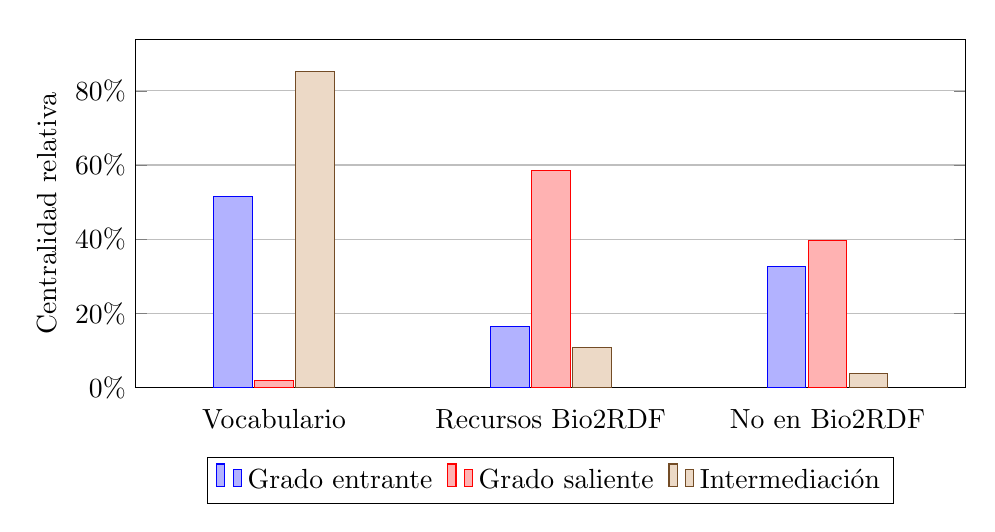
\begin{tikzpicture}
    \begin{axis}[
        width=\textwidth,height = 6cm,
        major x tick style = transparent,
        ybar=2*\pgflinewidth,
        bar width=14pt,
        ymajorgrids = true,
        ylabel = {Centralidad relativa},
        yticklabel={\pgfmathprintnumber{\tick}\%},
        symbolic x coords={Vocabulario,Recursos Bio2RDF,No en Bio2RDF},
        xtick = data,
        scaled y ticks = false,
        enlarge x limits=0.25,
        ymin=0,
        legend style={at={(0.5,-0.2)}, anchor=north,legend columns=-1}]
        \addplot coordinates {(Vocabulario, 51.51) (No en Bio2RDF, 32.72) (Recursos Bio2RDF, 16.44)};
        \addplot coordinates {(Vocabulario, 1.83)  (No en Bio2RDF, 39.62) (Recursos Bio2RDF, 58.54)};
        \addplot coordinates {(Vocabulario, 85.23) (No en Bio2RDF, 3.84)  (Recursos Bio2RDF, 10.92)};
        \legend{Grado entrante\,\,, Grado saliente\,\,, Intermediación};
    \end{axis}
  \end{tikzpicture}
  \caption{Centralidad relativa por tipo de dato.}
  \caption*{
    Según la intermediación los nodos más centrales se encontraron
    mayoritariamente en el vocabulario. Para la centralidad de grado
    saliente sin embargo la centralidad se acumuló en los recursos de Bio2RDF.
    Por su parte, la centralidad de grado entrante es aquella que posee valores
    más distribuidos entre el tipo de datos de los nodos.
  }
  \label{fig:comptype}
\end{figure}

Podemos notar como los resultados son los esperados para las centralidades de
grado.
Tiene sentido esperar que aquello sobre lo que se consulta sean las  drogas, por
ello la centralidad de grado saliente es tan alta para este tipo de recursos.
De la misma forma, la centralidad de grado entrante suele estar en el
vocabulario debido a que son las propiedades a consultar.
Teniendo esto en consideración, muchas consultas deben usar triples
como: \tt{?drug rdf:type drugbank\_vocabulary:Drug} y similares, que denotan la
busqueda de drogas (u otros) que cumplan con filtros adicionales.

Por su parte, la intermediación nos indica que los puntos clave de comunicación
están dentro del vocabulario, en especifico en la interacción droga a droga, la
cual, en una base de datos como DrugBank, es natural que sea importante.

\section{Conclusiones}\label{sec:con}
El proceso de obtención de datos, creación del grafo y cálculo de centralidad
realizados en este trabajo muestra tener gran eficacia. Menos de un $1\%$ de los
datos se perdieron en la creación de los mismos y el cálculo de centralidad
sobre el grafo generado se efectuó sin problemas. Si bien solo se trabajó con
los datos de DrugBank, el proceso es lo suficientemente genérico para ser
extendido a cualquier base de datos RDF.

Por su parte, los resultados del cálculo de centralidad evidencian la existencia
de relaciones claves dentro de DrugBank.
Como demuestran los resultados de intermediación y centralidad de grado
entrante, la interacción droga a droga (\tt{Drug-Drug-Interaction}) es sin duda
el nodo más importante de este vocabulario.

Se esperaba que las consultas utilizasen las relaciones del proyecto Bio2RDF e
información conjunta de todas las bases de datos, aún así, los resultados de
este trabajo no apuntan en esa dirección.
Las relaciones más centrales son exclusivamente del vocabulario interno de
DrugBank, es decir, para las consultas no se utilizan los enlaces generados por
el proyecto Bio2RDF, sino que los existentes en la base de datos seleccionada.
Este fenómeno parece indicar que a pesar de existir enlaces y recursos
genéricos, éstos no son utilizados por los usuarios, por lo cual no se
aprovecha el modelo de datos común que aporta Bio2RDF.
Este resultado refuerza una de las conclusiones de \cite{hu2015link}, que afirma
que si bien existen enlaces entre las diferentes bases de datos (las llamadas
\tt{x-relation}) la semántica de las entidades conectadas difiere dependiendo de
en que base de datos están.
Aún así, para verificar este problema es necesario ampliar el análisis
incluyendo más bases de datos que sean parte del proyecto.

Otro fenómeno interesante descubierto  gracias a este estudio es la importancia
que se le da a la fuente de los datos (\tt{source}).
Se descubrió que, en las consultas analizadas, gran parte de los datos hacen
referencia a dos aplicaciones informáticas: ChemAxon y ALOGPS.
Esta aplicaciones al parecer generan datos para DrugBank, estos datos luego son
consultados por los usuarios y estos requieren la fuente, ya sea explícitamente
o mediante el software que utilizan para la búsqueda.

Con respecto a la temática de las consultas y sus respuestas se encontró que el
gen ABCA1 presenta una gran centralidad. Este gen está encargado de la
regulación del colesterol por lo que no es sorpresa que sea tan relevante en las
consultas hechas a la base de datos, teniendo en consideración que las
enfermedades relacionadas a la obesidad son una de las principales causas de
muerte del mundo.
Este resultado, junto a la aparición de variadas drogas como los componentes con
mayor centralidad de grado saliente, demuestra que la base de datos está siendo
utilizada para lo que se pensó, la investigación biológica.

En resumen se tiene que, para los datos consultados por los usuarios a
DrugBank:
\begin{enumerate}
  \item
    Los recursos más centrales son parte del vocabulario interno de DrugBank.
    Se destaca la interacción droga a droga, las dosis y los tipos de datos.
  \item
    No se utilizan las relaciones e información genérica proveida por Bio2RDF.
  \item
    La fuente de los datos es un recurso muy utilizado, de ellas destacan
    aplicaciones informáticas como ChemAxon  y ALOGPS. Se intuye que muchas
    consultas fueron generadas por este tipo de aplicaciones.
  \item
    La investigación hecha en la fecha de estas consultas parece estar dirigida
    al combate de las enfermedades causadas por el colesterol.
  \item
    Una serie de drogas presentan una gran relevancia en las respuestas
    obtenidas, entre ellas se destaca el etanol, el ibuprofeno y el paracetamol.
\end{enumerate}

\subsection{Problemas encontrados}\label{sec:con:pr}
En el \bf{proceso de extracción}, para obtener los triples que conforman la base
de datos requerida por los usuarios, se ejecutaron todas las consultas.
Esta es una operación costosa y un gran parte de las respuestas estaban vacías.
Por otro lado, muchas consultas requerían los mismos datos y estos fueron
solicitados reiteradamente para ser borrados en pasos siguientes del proceso.

Obtener la base de datos mínima de manera eficiente resultó ser un problema que
no pudo ser solucionado en el desarrollo de este trabajo.
El proceso seguido fue prácticamente fuerza bruta pues los filtros utilizados
para reducir el número de consultas no fueron capaces de determinar si dos (o
más) de estas retornarían lo mismo antes de efectuarlas.

Por otra parte hubo un problema con la \bf{completitud del grafo.}
Muchos triples que podrían haber sido interesantes de analizar se perdieron en
la generación del grafo pues solo se utilizó DrugBank como base de datos
objetivo.

Consultas que hacían uso intensivo de DrugBank puede que hallan resultado vacías
por requerir tan sólo un dato de otra fuente.
Lamentablemente hacer un cálculo teniendo en cuenta todas las fuentes generaría
cantidades de datos no procesables por la maquina en la que se trabajó.

Por último tenemos al \bf{tiempo del cálculo.}
Si bien el algoritmo utilizado es paralelo y generalmente eficiente, el grafo
sobre el cual se ejecutó es innecesariamente grande. 
Se generó un grafo muy disperso, con muchos sub-grafos disjuntos, que aportan
nada a los resultados de centralidad y ralentizaron el proceso innecesariamente.

Posibles soluciones a este problema serían la utilización de técnicas
incompletas para generar una estimación de la centralidad total, o el
pre-procesamiento del grafo de forma que se eliminen los nodos inútiles.

\subsection{Trabajo futuro}\label{sec:con:tf}
Se espera que este trabajo se tome como precedente para la investigación sobre
centralidad en bases de datos RDF.
Particularmente para el proyecto Bio2RDF la extensión natural será ampliar el
espectro de datos estudiados. Agregar más bases de datos pertenecientes al
proyecto logrará generar mejores estadísticas sobre la conectividad de los datos
de diferentes dominios y verificar la utilización de los enlaces generados.

Por otro lado, trabajos recientes como el de Garrido 
\etal\cite{garrido2016group} señalan a la centralidad de grupo (\emph{group
centrality}) como una forma interesante de medir la centralidad para un grafo
RDF.
Como su nombre lo indica, se basa en calcular la centralidad para
grupos de nodos, como resultado obtendremos las n-tuplas más centrales y no los
individuos particulares, de esta forma lograremos identificar de mejor manera
como se están haciendo las consultas y la relación entre los datos.
Este proceso no cambia la forma en la que se mide la
centralidad sino que sobre qué la medimos y por ello los algoritmos descritos
en este trabajo funcionarán correctamente.
Puede ser interesante generar esta métrica sobre los datos de Bio2RDF.

Por último, una mejora evidente en el calculo de centralidad está sujeta al tipo
de paralelización realizada. En \cite{madduri2009faster} se presentan algoritmos
más eficientes que el usado en este trabajo, pero requieren de una arquitectura
de procesador especial de la cual no disponemos.
Otra forma de hacer el trabajo más eficiente es no calculando la intermediación
completamente, sino que obteniendo una estimación de ella por caminos
aleatorios o métodos similares.
